% !TeX root = ../dissertation.tex

\chapter{Modelling in Imitator}


To explore the capabilities of the Imitator tool in greater detail, we begin by thoroughly defining its syntax, outlining the process of building a complete model in Imitator (Section~\ref{sec:specifying_automata}).
\todo{refer to sections 3.2 and 3.3}%
The rest of this chapter describes how to use Imitator using four real-time systems (Section~\ref{sec:examples}): a \emph{Traffic Light System}, a \emph{Coffee Machine}, a \emph{Worker Hammer System} and a simple \emph{ATM Machine}. For each system, parameter synthesis will be demonstrated by verifying parameter constraints to prevent deadlocks. Additionally, one of the parameters in each system will be optimized.

\section{Specifying automata}\label{sec:specifying_automata}

The Imitator tool can always be divided into three main parts. In each part, the worker automaton from the worker and hammer example presented in Chapter 2 will be used to illustrate the Imitator's syntax.

\newcommand{\kw}[1]{\texttt{\textbf{\textcolor{blue!80!black}{#1}}}}

\begin{itemize}
    \item \textbf{Variable declarations}

    % \begin{figure}[H]
    % \centering
    \begin{lstlisting}[language=UPPAAL, caption={Variable Declaration Exemple using Worker Automata}, label={lst:VD_example_1}, float={bt}]
    var   session, t             : clock;
          sessionTime, reactTime : parameter;   
    \end{lstlisting}
    % \end{figure}

    In the variable declaration block, illustrated in Listing~\ref{lst:VD_example_1},
    we define the essential elements of the model, including \kw{clock}s, discrete variables, \kw{constant}s, and \kw{parameter}s. These elements are used in expressions that represent temporal constraints in the rest of the model.

    The \kw{clock}s are special variables that can evolve continuously, all at the same rate.
    % and the way to declare them is with the suffix \textbf{: clocks} after defining their names.
    Traditional variables are discrete and have an assigned type, which can be \kw{Int} (integer), \kw{Boolean}, \kw{Array}, etc., written e.g. \texttt{x : \kw{Int}} for an integer variable. Only discrete variables can be shared among different automata. Variables marked with \kw{constant} cannot be modified.
    Finally, a \kw{parameter} is an undefined variable that is inferred automatically by Imitator, which will be explained later.

    % Both are shared by all automata in the model and, unlike discrete variables, the value of global ones cannot be altered. Within discrete variables, there are several types, such as: Integers (Int), Booleans, Arrays, Lists, Stacks, and Queues. Just like with clocks, to declare these variables, you simply use the suffix \textbf{: Type}, where 'Type' represents the desired type from the ones mentioned earlier.

    % We can see an example of the variable declaration in Listing \ref{lst:VD_example}.



    \item \textbf{Automata}

    In the Automata block, we define the timed automata that represent the system's behavior. It includes states, which represent different phases of the system, and transitions, which define how the system moves from one state to another. Additionally, it contains invariants, which impose constraints on the time that can be spent in a state, guards, which set conditions for a transition to occur, and assignments, which update variables or clocks after a transition.

    Before constructing the automaton, it is necessary to explicitly declare all the synchronization actions present in the model using the keyword \kw{synclabs}, followed by the corresponding transitions.

    Each location of the automaton is initialized with \kw{loc}, followed by its name and, if present, an invariant. The definition continues with \kw{when}, followed by the transition condition, \kw{sync} for the synchronization action, \kw{do} for variable or clock updates, and \kw{goto} to indicate the next state. If there are multiple transitions from the same location, they are listed sequentially.

    Each location can be urgent if no time passage is allowed in that location, defined by the keyword \kw{urgent}. This means the system must leave this location immediately without allowing time to elapse. A location can be accepting if it represents a significant final state for verifying liveness properties. Accepting locations are used to define states that must be reached repeatedly in infinite executions, making them useful for checking the recurrence of desired behaviors. It is defined by the keyword \kw{acepting}.
    Additionally, a location can combine both properties, being both urgent and accepting, ensuring that the system reaches this location without delay and that it is considered for acceptance conditions in liveness verification.

    It is also worth noting that the keyword \kw{Stop} allows certain clocks to be interrupted in specific locations, while \kw{Flow} enables the modification of the clock's evolution rate.

    

    \begin{figure}[H]
    \centering
    \begin{lstlisting}[language=UPPAAL, caption={Construction of the Automata using Worker Automata as Example}, label={lst:VD_example}]
    (*Worker Automata*)
    automaton Worker
    
    synclabs: rest, hit, newNail, Work;
    
    loc Rest: invariant session <= sessionTime - reactTime
      	when True sync Work do {t := 0} goto Work;
    
    loc Work: invariant session <= sessionTime && t <= reactTime
      	when t >= reactTime sync newNail do {t := 0} goto Work;
      	when t >= reactTime - 5 sync hit do {t := 0} goto Work;
      	when session >= sessionTime sync rest do {session := 0} goto Rest;
    
    end	(* Worker *)
    \end{lstlisting}
    \end{figure}

    

    
    \item \textbf{Initial state definition}

    The initial state definition section is split between the discrete initialization and the continuous initialization. This section starts with the keyword \kw{init}, with each condition separated by \kw{\&}.
    The discrete initialization (optional introduced by the discrete keyword) assigns an initial value to each discrete variable, and sets the initial location for each automaton.
     The continuous initialization (optional introduced by the continuous keyword) defines the initial constraints over clocks and parameters (possibly also using discrete variables).

    \begin{figure}[H]
    \centering
    \begin{lstlisting}[language=UPPAAL, caption={Initial state definition using Worker Automata as Exemple}, label={lst:VD_example}]
    init := loc[Worker] = Rest
          & session = 0
          & t = 0
          & sessionTime >= 0
          & reactTime >= 0;
    end (* of file *)
    \end{lstlisting}
    \end{figure}
    
\end{itemize}
% \paragraph{}

\section{Specifying queries}
%explicar ficheiro separado e exemplificar prop anteriores


Finally, in terms of the syntax of the queries, which, as explained earlier, are written in a separate file, the query consists of the synthesis mode (synth or witness) and the synthesis algorithm. This condition is known as a state predicate that defines a specific state of an automaton. It typically takes the form loc[AUTOMATON] = LOCATION, where AUTOMATON is the name of the automaton and LOCATION is the name of a location within it. State predicates support logical operations like conjunction (AND), disjunction (OR), and can also involve global discrete variables \cite{IMITATOR}. The query is stored in a separate file with the \texttt{.imiprop} extension.

To check if the system is syntactically correct and in the desired format, we save the code in a file with the .imi extension (e.g., system.imi). Then, we execute the following command in the terminal: \texttt{./imitator system.imi [hammer\_proprities.imiprop]}. The system.imi file serves as a model, representing various systems. Alongside, the property.imiprop file contains all the properties that we aim to check. The -option flag in the command line allows to specify the desired output file format, whether it be PNG, Uppaal, or any other preferred format. It's important to note that the parameters enclosed in square brackets are optional~\cite{IMITATOR}.

\section{Installing Imitator}
The easiest and fastest way to install Imitator is by using Docker. Other alternatives can be found online at \url{https://www.imitator.fr/}. You can download the Imitator docker image with the following command: \texttt{docker pull imitator/imitator}. The developers of Imitator recommended to run the container from a bash terminal using a shared directory with the host computer. This facilitates extracting the results from using Imitator within the Docker image.
% the interaction with the imitator's binaries an the documents, as any changes made inside the container are reflected directly in the directory on your computer.
The container will be automatically removed once it is closed when using the option \texttt{--rm}. Summarising, we use the following command to run Imitator over a file called 
\texttt{docker run --rm -it --entrypoint
/usr/bin/bash -v Directory Path/Directory Name imitator/imitator}.

In the next chapter, as will be explained, the command used in the Backend is quite similar, with the interactive option (-it) removed, resulting in: \texttt{docker run --rm --entrypoint /usr/bin/bash -v Directory Path/Directory Name imitator/imitator}.


\section{Examples}\label{sec:examples}

We illustrate the syntax defined above with three examples:
% With the syntax defined, we now move on to the examples, as previously mentioned. Three examples will be presented:
a \emph{Coffee Machine}, a \emph{Worker and Hammer System}, and a \emph{ATM Machine}. For each system a set of properties will be tested to demonstrate the capabilities of the Imitator tool.

\begin{comment}

    
\subsection{Traffic Light System}

First, we have a system where two roads intersect at a right angle: one is Road A, and the other is Road B. Both roads are one-way, meaning vehicles can only move in a specific direction. To ensure smooth traffic flow and prevent accidents, traffic lights control the intersection. These traffic lights allow vehicles traveling on Road B to merge onto Road A without issues, ensuring an organized and safe flow of traffic. The situation is better descrived in Figure \ref{fig:sinal}.
\vspace{0.5cm}

\begin{figure} [H]
    \centering
    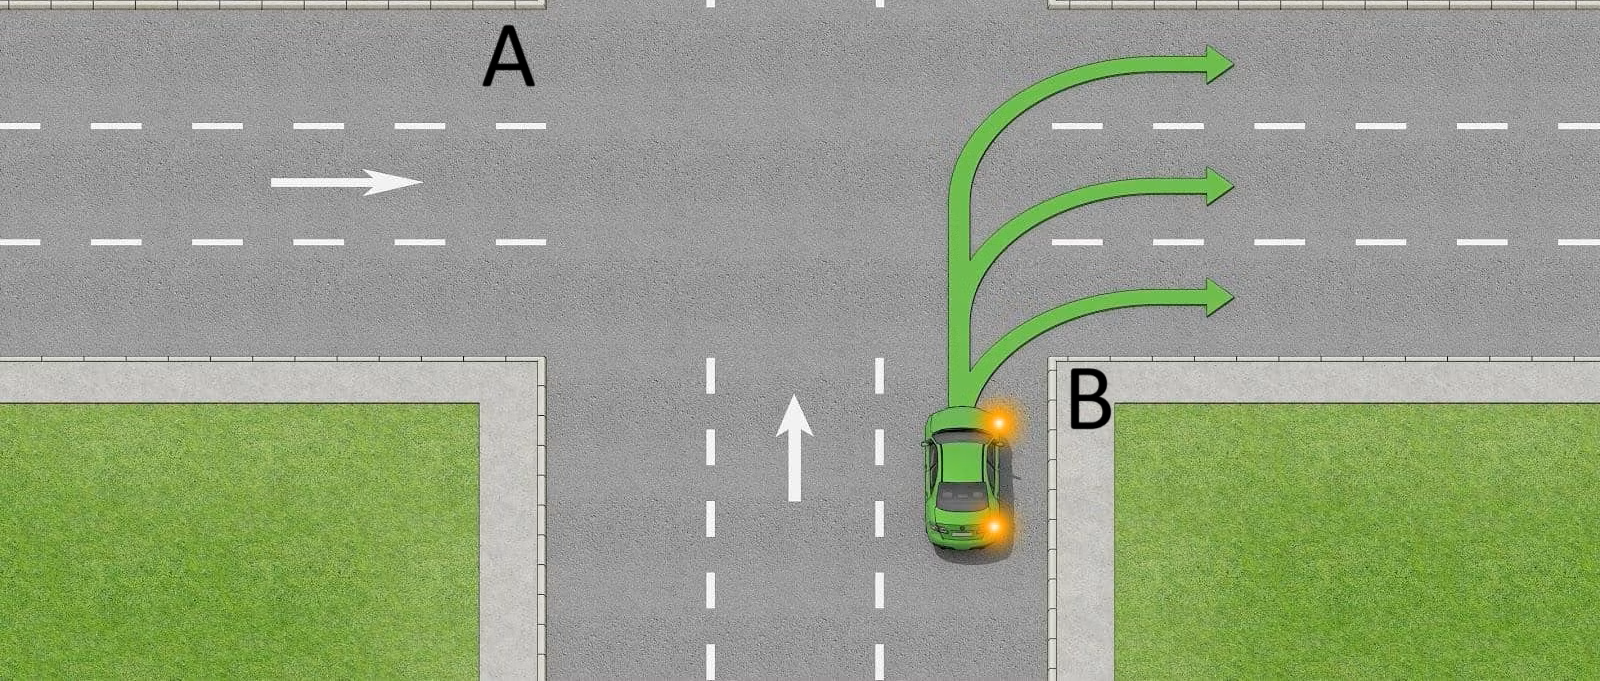
\includegraphics[width=0.75\linewidth]{images/Estrada_3.png}
    \caption[Traffic control of two roads by a traffic light.]{Traffic control of two roads by a traffic light~\cite{Abate2021}.}
    \label{fig:sinal}
\end{figure}

To translate this system into the IMITATOR syntax, it is necessary to represent events and transitions over time using concepts such as \textbf{clocks}, \textbf{variables}, \textbf{states}, and \textbf{transitions}. As explained in the previous chapter, to build our model, we need to construct three essential blocks.

In the first block, we declare the clocks and variables (discrete, rational, or parameters), as shown in Listing \ref{lst:traffic_var}.

\begin{figure}[H]
    \centering
    \begin{lstlisting}[language=UPPAAL, caption={Annotation Block rewritten with new values}, label={lst:traffic_var}]
    var
    x1, x2 : clock;
    
    T1_Green : parameter;
    T2_Green : parameter;
    T1_Yellow : parameter;
    T2_Yellow : parameter;
    T1_Red : parameter;
    T2_Red : parameter; 
    \end{lstlisting}
\end{figure}



The variables \texttt{x1} and \texttt{x2} are the internal counters of each traffic light, while the parameters, i.e., the variables, represent the thresholds for the duration each light can stay in each color. In this example, these times are not specifically defined, allowing the tool to optimize them as needed.


The next step is to construct the automata, defining their behavior using the previously declared clocks and variables. To improve readability, the automaton for Traffic Light 1 (Listing \ref{lst:sem_1}) is presented separately from the automaton for Traffic Light 2 (Listing \ref{lst:sem_2}).

%\begin{figure}[H]
%    \centering
    \begin{lstlisting}[language=UPPAAL, caption={Annotation Block rewritten with new values}, label={lst:sem_1}]
    (* Traffic Light 1 *)
    automaton Sem1
    synclabs: Go_Y;
    
    loc Green1:
      invariant x1 <= T1_Green
      when x1 = T1_Green sync Go_Y do {x1 := 0} goto Yellow1;
    
    loc Yellow1:
      invariant x1 <= T1_Yellow
      when x1 = T1_Yellow do {x1 := 0} goto Red1;
    
    loc Red1:
      invariant x1 <= T1_Red
      when x1 = T1_Red sync Go_Y do {x1 := 0} goto Green1;
    
    end
    \end{lstlisting}
%\end{figure}



%\begin{figure}[H]
%    \centering
    \begin{lstlisting}[language=UPPAAL, caption={Annotation Block rewritten with new values}, label={lst:sem_2}]
    (* Traffic Light 2 *)
    automaton Sem2
    synclabs: Go_Y;
    
    loc Green2:
      invariant x2 <= T2_Green
      when x2 = T2_Green sync Go_Y do {x2 := 0} goto Yellow2;
    
    loc Yellow2:
      invariant x2 <= T2_Yellow
      when x2 = T2_Yellow do {x2 := 0} goto Red2;
    
    loc Red2:
      invariant x2 <= T2_Red
      when x2 = T2_Red sync Go_Y do {x2 := 0} goto Green2;
    
    end
    \end{lstlisting}
%\end{figure}

\paragraph{}

Two automata have been declared, one for each traffic light. The behavior of both is very similar: in each state (green, yellow, red), there is an invariant condition that ensures the time each traffic light stays in each color will not be exceeded. Since the time values are parameters, they do not yet have a concrete value defined.

When the time limit for traffic light A's color is reached, the guard condition is triggered, initiating the color alternation between the two traffic lights. This resets both timers, synchronizing the transition of traffic light B, even if, in this case, the guard condition has not been directly validated.We can think of traffic light A as the master and traffic light B as the slave, ensuring that they can never be red or green simultaneously.

To better understand and summarize the model, we have constructed transition tables that represent the different system states, the invariants associated with each state, the conditions required for a transition to occur (guards), the synchronization events that trigger state changes, and the resulting next state for each transition. These tables provide a clear visualization of the automaton's logic, making it easier to analyze the system's behavior and ensuring that all timing constraints and synchronization events are properly followed.

\begin{table}[h!]
\centering
\begin{tabular}{|l|l|l|l|l|}
\hline
\textbf{State}  & \textbf{Invariant}      & \textbf{Guard}          & \textbf{Synchronized Event} & \textbf{Next State} \\ \hline
\texttt{Green1}  & $x_1 \leq T1\_Green$   & $x_1 = T1\_Green$       & \texttt{Go\_Y}        & \texttt{Yellow1}   \\ \hline
\texttt{Yellow1} & $x_1 \leq T1\_Yellow$  & $x_1 = T1\_Yellow$      & None                     & \texttt{Red1}      \\ \hline
\texttt{Red1}    & $x_1 \leq T1\_Red$     & $x_1 = T1\_Red$         & \texttt{Go\_Y}        & \texttt{Green1}    \\ \hline
\end{tabular}
\caption{Transition table for Traffic Light 1 (Sem1)}
\end{table}

\begin{table}[h!]
\centering
\begin{tabular}{|l|l|l|l|l|}
\hline
\textbf{State}  & \textbf{Invariant}      & \textbf{Guard}          & \textbf{Synchronized Event} & \textbf{Next State} \\ \hline
\texttt{Green2}  & $x_2 \leq T2\_Green$   & $x_2 = T2\_Green$       & \texttt{Go\_Y}        & \texttt{Yellow2}   \\ \hline
\texttt{Yellow2} & $x_2 \leq T2\_Yellow$  & $x_2 = T2\_Yellow$      & None                     & \texttt{Red2}      \\ \hline
\texttt{Red2}    & $x_2 \leq T2\_Red$     & $x_2 = T2\_Red$         & \texttt{Go\_Y}        & \texttt{Green2}    \\ \hline
\end{tabular}
\caption{Transition table for Traffic Light 2 (Sem2)}
\end{table}

\paragraph{}

Finally, we need to declare the initial positions of each automaton, initialize the variables, and set limits for them or for the timers (if applicable):

% \begin{lstlisting}[language=UPPAAL]
%     init := {
%         discrete = 
%             (*INITIAL LOCATION*)
%             loc[Sem1] := Green1,
%             loc[Sem2] := Red2,
    
%         ;
%         continuous =
%             (*INITIAL CLOCKS*)
%             & x1 = 0
%     	       & x2 = 0
            

%             (*PARAMETER CONSTRAINTS*)
%             & T1_Green > 0
%             & T2_Green > 0
%             & T1_Yellow > 0
%             & T2_Yellow > 0
%             & T1_Red > 0
%             & T2_Red > 0
%     	       & T1_Green = T2_Green + 60
%         ;

%     }
% \end{lstlisting}

\begin{lstlisting}[language=UPPAAL]
    init :=
            (*INITIAL LOCATION*)
          & loc[Sem1] := Green1
          & loc[Sem2] := Red2
            (*INITIAL CLOCKS*)
          & x1 = 0
          & x2 = 0
            (*PARAMETER CONSTRAINTS*)
          & T1_Green > 0
          & T2_Green > 0
          & T1_Yellow > 0
          & T2_Yellow > 0
          & T1_Red > 0
          & T2_Red > 0
          & T1_Green = T2_Green + 60;
\end{lstlisting}



\paragraph{}
As explained in the previous chapter, this part of the code is subdivided into discrete and continuous sections. It is important to highlight that, in the continuous part, an extra condition is added to the parameters: they must not only be greater than 0, but also the time that traffic light 1 stays green must be at least one minute longer than the time that traffic light 2 stays green.

As in the previous examples, we convert our model code into a visual representation as we can see in the Figure \ref{fig:TF_PTA}.

\paragraph{}

\begin{figure} [H]
    \centering
    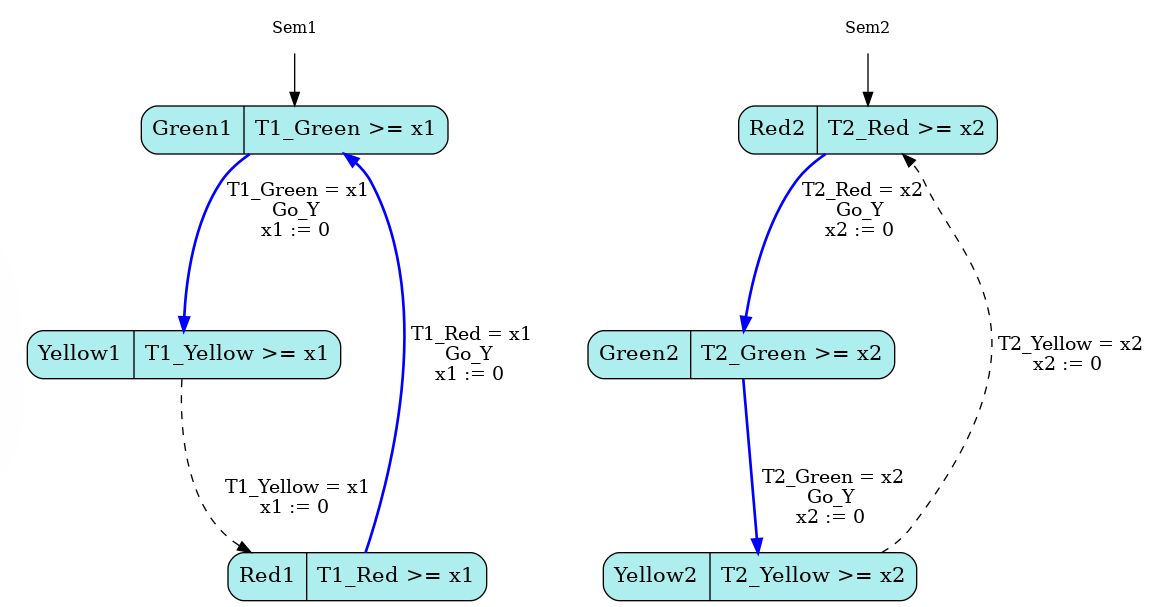
\includegraphics[width=1.05\linewidth]{images/Sem_pta.png}
    \caption[Traffic Light Automata]{Traffic Light Automata}
    \label{fig:TF_PTA}
\end{figure}

%\subsubsection{System Analysis}

%Com o modelo construído procedemos á verificação das propriedades tal como no exemplo anterior e já tendo as propriedades guardadas num ficheiro .imiprop separado do modelo. Começamos pela verificação da não ocorrência de deadlock sendo que usamos a seguinte syntax : property := synth DeadlockFree;




\paragraph{}
\paragraph{}
\end{comment}

\subsection{Coffee Machine}

First, we have a Coffee Machine system. To simplify, it is assumed that this machine does not require coins or any other mechanism to start the process; it only has 1 button to initiate the process. This button is also used to add sugar to the coffee.

\begin{figure} [H]
    \centering
    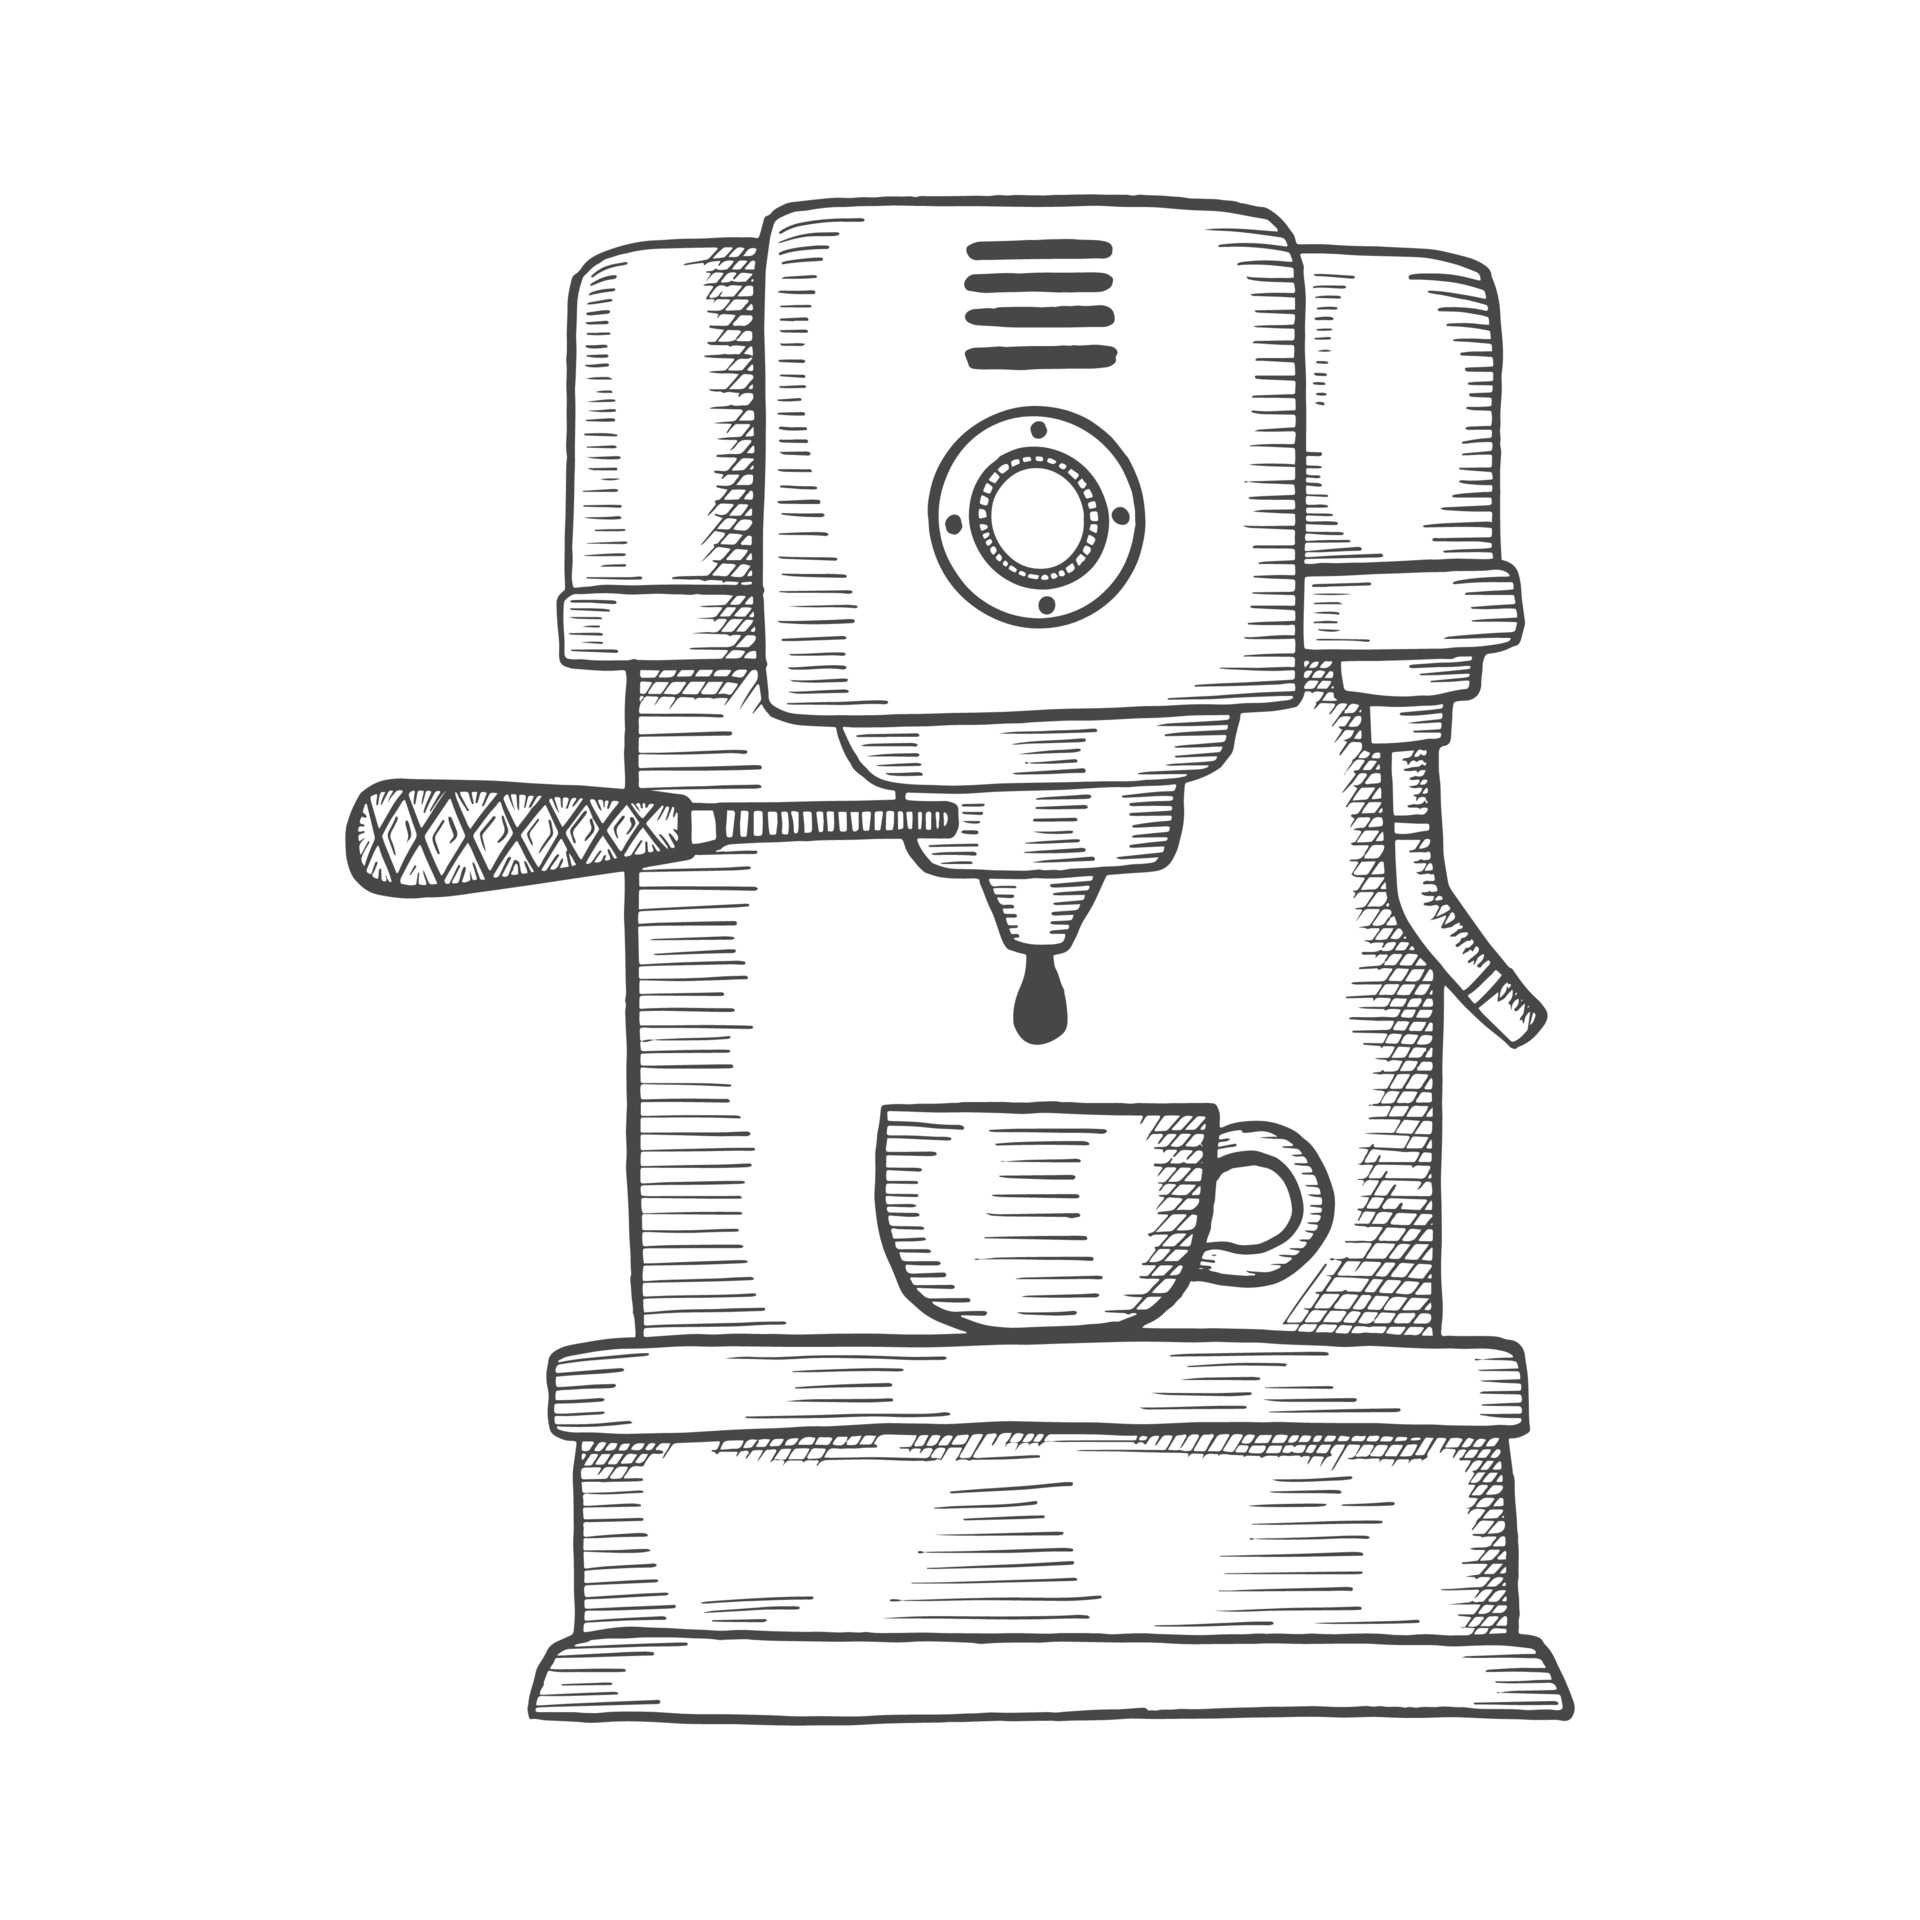
\includegraphics[width=0.4\linewidth]{chapters/vecteezy_coffee-espresso-machine-lover-single-isolated-hand-drawn_8148187.jpg}
    \caption[Simple Coffee Machine with only one button to control all operations.]{Simple Coffee Machine with only one button to control all operations.~\cite{Abate2021}}
    \label{fig:modelcheckingC}
\end{figure}

\paragraph{}

To translate this system into the IMITATOR syntax, it is necessary to represent events and transitions over time using concepts such as \textbf{clocks}, \textbf{variables}, \textbf{states}, and \textbf{transitions}. As explained in the previous chapter, to build our model, we need to construct three essential blocks.

In the first block, we declare the clocks and variables (discrete, rational, or parameters):

\begin{lstlisting}[language=UPPAAL]
    var  x, y       : clock;
         p1, p2, p3 : parameter;
\end{lstlisting}

The variable \textbf{p1} represents the time elapsed between two consecutive sugar requests after the process has started. In other words, it is the interval between each request made by the user to add sugar to the coffee. The variable \textbf{p2} defines the time window during which the user can press the button again to request more sugar. If the system allows this additional request, it will wait for user interaction within this interval before proceeding with the process. Finally, the variable \textbf{p3} corresponds to the time required to produce and serve the coffee. This period includes all steps from the beginning of the preparation until the moment the beverage is served to the user.

\paragraph{}

The next step is the construction of the automaton. In this case, a single automaton will be developed to represent the operation of the coffee machine.

\begin{lstlisting}[language=UPPAAL]
    (*Coffe Machine*)
    synclabs: press, cup, coffee, sleep;

    loc idle: invariant True
    	when True sync press do {x := 0, y := 0} goto add_sugar;
    
    loc add_sugar: invariant y <= p2
    	when x >= p1 sync press do {x := 0} goto add_sugar;
    	when y = p2 sync cup do {} goto preparing_coffee;
    
    loc preparing_coffee: invariant y <= p3
    	when y = p3 sync coffee do {x := 0} goto cdone;
    
    accepting loc cdone: invariant x <= 10
    	when True sync press do {x := 0, y := 0} goto add_sugar;
    	when x = 10 sync sleep goto idle;
    
    end
\end{lstlisting}


The coffee machine's automaton consists of four states. The first state is \textbf{Standby(\textit{idle})}, where the system waits indefinitely for the user to take action to start making coffee. The next state is \textbf{\textit{add\_sugar}}, where the user can choose to add sugar. There is a time limit (p₂) for adding sugar, and a restriction (p₁) on how often sugar can be added in quick succession. These restrictions are enforced using invariants, in the state add\_sugar, with the invariant y ≤ p₂ and in the preparing\_coffee state with the invariant y ≤ p₁.The synchronization here is based on the \textit{press} event, which triggers the action of adding sugar and starts the process. Next is the coffee preparation state\textbf{(\textit{preparing\_coffee})}, which takes p₃ time units to complete. The synchronization with the coffee event triggers the completion of the coffee preparation. Finally, in the last state(\textbf{\textit{cdone}}), if the user presses the button again within 10 time units, the system goes back to add\_sugar and repeats the process. This synchronization is triggered by the \textit{press} event. If the user does not press the button within the allowed time, the system synchronizes with the \textit{sleep} event, returning to the Standby state.

It is important to note that the last state, called the \textbf{\textit{accepting loc}}, is different from the others because it represents a 'final' or 'accepting' state. In simple terms, once the system reaches this state, the coffee is prepared and ready to be served. This distinction is useful during the verification process, as it allows us to check whether the automaton can reach a successful end state instead of getting stuck in infinite loops within intermediate states \cite{IMITATOR}.

The model is summarized in Transition Table \ref{tab:automato_cafe}.

\paragraph{}



\begin{table}[h!]
\centering
\resizebox{\textwidth}{!}{
\begin{tabular}{|l|l|l|l|l|l|}
\hline
\textbf{State}             & \textbf{Invariant}     & \textbf{Guard}         & \textbf{Synchronized Event} & \textbf{Action}              & \textbf{Next State}       \\ \hline
\texttt{idle}              & Always (\texttt{True})  & Always (\texttt{True}) & \texttt{press}        & \texttt{x := 0, y := 0}  & \texttt{add\_sugar}       \\ \hline
\texttt{add\_sugar}        & $y \leq p_2$           & $x \geq p_1$           & \texttt{press}        & \texttt{x := 0}          & \texttt{add\_sugar}       \\ \hline
\texttt{add\_sugar}        & $y \leq p_2$           & $y = p_2$              & \texttt{cup}          & None           & \texttt{preparing\_coffee} \\ \hline
\texttt{preparing\_coffee} & $y \leq p_3$           & $y = p_3$              & \texttt{coffee}       & \texttt{x := 0}          & \texttt{cdone}            \\ \hline
\texttt{cdone} & $x \leq 10$            & Always (\texttt{True}) & \texttt{press}        & \texttt{x := 0, y := 0}  & \texttt{add\_sugar}       \\ \hline
\texttt{cdone}            & $x \leq 10$            & $x = 10$               & \texttt{sleep}        & None           & \texttt{idle}             \\ \hline
\end{tabular}
}
\caption{Transition table of the coffee machine automaton.}
\label{tab:automato_cafe}
\end{table}



To complete the model, it is necessary to declare the initial states as well as the possible constraints on the clocks and declared variables:

\begin{lstlisting}[language=UPPAAL]
    init :=
    	(* Initial location *)
    	& loc[machine] = idle
    	(* Initial clock constraints *)
    	& x = 0
    	& y = 0
    	(* Parameter constraints *)
    	& p1 >= 0
    	& p2 >= 0
    	& p3 >= 0
    ;
\end{lstlisting}



The initial location, as explained earlier, is set to the \textit{idle} state, meaning Standby mode. Additionally, the clocks are initialized to 0, and the parameters must be positive.

\paragraph{}

To verify whether our system complies with the syntax, we can, as explained in the previous chapter, run the model in the command line with the option to translate the system into a PNG image using the following command: \texttt{./imitator mod.imi -imi2PNG}

If this command fails, it means that our model has syntax errors that need to be fixed.

Considering that we saved our model in the \textbf{mod.imi} file, we obtain the following image as output in Figure \ref{fig:cof_output}, which visually represents our code.




\begin{figure} [H]
    \centering
    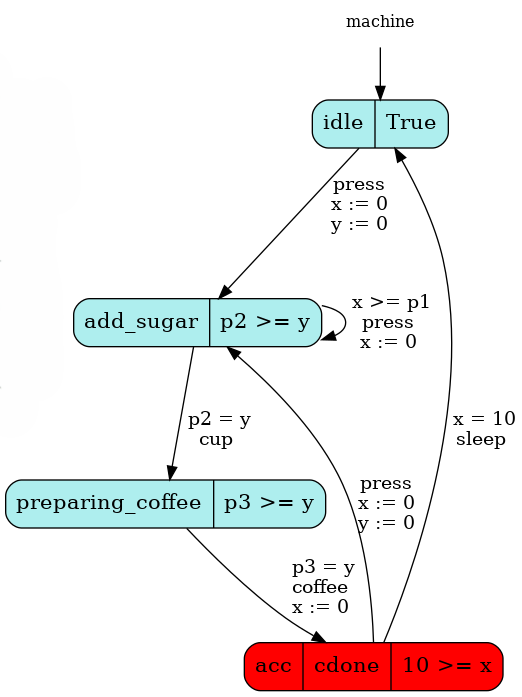
\includegraphics[width=0.55\linewidth]{images/sys.png}
    \caption[Coffee Machine Automata]{Coffee Machine Automata}
    \label{fig:cof_output}
\end{figure}




\subsubsection{System Analysis}

Once the model is built, we can proceed to property verification. We start with parameter synthesis to ensure that deadlocks are avoided. To achieve this, we need to create a separate \texttt{.imiprop} file, distinct from the .imi file containing our model, as explained in the previous chapter.


Inside the file, we define the property to be verified. In this case, related to deadlock. The syntax is as follows : \texttt{property := \#synth DeadlockFree;}

The result is stored in a \texttt{.res} file with the same name as the file where the model is saved. This file contains general information about the model as well as the verification of the property. However, the most important part we extract is the following:

\begin{verbatim}
     p1 >= 0
    & p2 >= 0
    & p3 >= p2
    OR
      p2 > p3
    & p3 >= 0
    & p1 = 0
\end{verbatim}

Any values chosen for the parameters, as long as they satisfy the given constraint, ensure that the system does not reach a deadlock. We can also determine the maximum or minimum parameter value that ensures a given property is satisfied. For example, we may want to find the shortest possible time between two consecutive sugar requests(\( p1 \)) while still allowing the coffee to be served to the user (i.e., reaching the location \texttt{cdone}).

To achieve this, we can use the following property: 
\texttt{property := \#synth EFpmin(loc[machine] = cdone, p1);} With this property, we obtain the following result:

\begin{verbatim}
     p3 >= p2
     & p2 >= 0
     & p1 = 0
\end{verbatim}

The parameter \( p1 \) can be 0, meaning that the request for sugar can be made instantly. However, this is only possible as long as the time required to prepare a coffee (\( p1 \)) is greater than the time interval in which sugar can be requested (\( p2 \)). Additionally, \( p2 \) must be strictly positive to ensure a valid sequence of events.

A synthesis of both verified properties can be found in the table \ref{tab:property_results}

\begin{table}[h!]
\centering
\resizebox{\textwidth}{!}{
\begin{tabular}{|p{5cm}|l|p{5cm}|}
\hline
\textbf{Property} & \textbf{Meaning} & \textbf{Result} \\ \hline
\texttt{property := synth DeadlockFree;} & Ensures the system does not reach a deadlock state. & 
\begin{minipage}[t]{8cm}
$p_1 \geq 0 \land p_2 \geq 0 \land p_3 \geq p_2$\\
\textbf{or}\\
$p_2 > p_3 \land p_3 \geq 0 \land p_1 = 0$
\end{minipage} \\ \hline

\texttt{property := \#synth EFpmin(loc[machine] = cdone, p1);} & Finds the minimum value of $p_1$ to reach location \texttt{cdone}. &
\begin{minipage}[t]{8cm}
$p_3 \geq p_2$\\
$p_2 \geq 0$\\
$p_1 = 0$
\end{minipage} \\ \hline
\end{tabular}
}
\caption{Synthesis of properties and corresponding results.}
\label{tab:property_results}
\end{table}


\subsection{Worker and Hammer System}

Now we have the "Worker and Hammer" system, as discussed in the State of the Art chapter and implemented in UPPAAL. This system represents the interaction between a worker and a hammer to perform a repetitive task, such as hammering nails.

As in the other examples, we start by defining the variables and clocks of the automata.

\begin{lstlisting}[language=UPPAAL]
    var
    session, t
    :clock;
    
    sessionTime,
    reactTime,
    totalNails
    : parameter;
    nails
    : int;	
\end{lstlisting}


The \textbf{t} and \textbf{session} timers are used to measure elapsed time for different purposes. The t timer tracks short-duration actions, such as hammering a nail or placing a new one, while the session timer records the total time a worker has spent working in a session, determining when the worker need to take a break. The variables \textbf{sessionTime}, \textbf{reactTime}, and \textbf{totalNails} are defined as parameters, unlike in the UPPAAL example, where they had fixed values. \textbf{sessionTime} represents the maximum time a worker can work before stopping, \textbf{reactTime} is the maximum time allowed for the worker to hit or place a new nail, and \textbf{totalNails} indicates the total number of new nails available. Finally, the variable \textbf{Nails} is defined as a discrete type, specifically an integer, and serves as an accumulator for the number of completed nails. Its value is initialized to 0 in the final section of the code. With all variables declared, the next step is the definition of the automata.
%\paragraph{}

\begin{lstlisting}[language=UPPAAL]
    (*Worker Automata*)
    automaton Worker
    
    synclabs: rest, hit, newNail, Work;
    
    loc Rest: invariant session <= sessionTime - reactTime
      	when True sync Work do {t := 0} goto Work;
    
    loc Work: invariant session <= sessionTime && t <= reactTime
      	when t >= reactTime sync newNail do {t := 0} goto Work;
      	when t >= reactTime - 5 sync hit do {t := 0} goto Work;
      	when session >= sessionTime sync rest do {session := 0} goto Rest;
    
    end
    
    (*Hammer Automata*)
    automaton Hammer
    
    synclabs: hit, newNail;
    
    loc NailUp: invariant True
      	when True sync hit goto NailHalf;
    
    loc NailHalf: invariant True
      	when True sync hit do {nails := nails +1} goto NailDone;
    
    loc NailDone: invariant True
      	when nails <= totalNails sync newNail goto NailUp;
    
    end


\end{lstlisting}


The system consists of two automata: \textbf{Worker} and \textbf{Hammer}. The \textbf{Worker} represents a worker who alternates between the states Rest and Work. In the Rest state, the worker waits for the start of work through the Work synchronization, resetting the clock t in the process. After this synchronization, in the Work state, the worker can perform two actions: hitting the nail (hit), if t ≥ reactTime - 5, or placing a new nail (newNail!), if t ≥ reactTime, always resetting t after each action. The worker can remain in the Work state as long as session < sessionTime. Once this limit is exceeded, the worker returns to the Rest state through the transition rest!, which also resets the session clock.

The \textbf{Hammer} automaton represents the interaction of the hammer with the nails, alternating between the states NailUp (new nail), NailHalf (partially hammered nail), and NailDone (completely hammered nail). Initially, it is in the NailUp state, where upon receiving the synchronization Hit, it transitions to NailHalf. Upon receiving a second synchronization Hit, it transitions to NailDone, incrementing the variable nails if countNails is activated. When the nail is completely hammered, the system can insert a new nail through the synchronization newNail?, returning to the NailUp state, provided that infiniteNails is true or nails < totalNails. 

The synchronization between the two automata occurs through the channels Hit and newNail presented in the Worker and Hammer automata, ensuring that the sequence of events is consistent and respects the temporal constraints imposed by the clocks t and session.

We can better visualize the behavior of the Worker automaton in Table \ref{tab:wh_t1} and of the Hammer automaton in Table \ref{tab:wh_t2}.
\paragraph{}

\begin{table}[h!]
\centering
\resizebox{\textwidth}{!}{
\begin{tabular}{|l|l|l|l|l|l|}
\hline
\textbf{State}             & \textbf{Invariant}            & \textbf{Guard}                & \textbf{Synchronized Event} & \textbf{Action}               & \textbf{Next State}         \\ \hline
\texttt{Rest}              & Always (\texttt{True})         & session $\leq$ sessionTime - reactTime & \texttt{work!}              & \texttt{session := 0}         & \texttt{Work}               \\ \hline
\texttt{Work}              & session $\leq$ sessionTime     & t $\leq$ reactTime            & \texttt{newNail!}            & \texttt{t := 0}               & \texttt{Work}               \\ \hline
\texttt{Work}              & session $\leq$ sessionTime     & t $\geq$ reactTime - 5        & \texttt{hit!}                & \texttt{t := 0}               & \texttt{Work}               \\ \hline
\texttt{Work}              & session $\geq$ sessionTime     & None                              & \texttt{rest!}               & \texttt{session := 0}         & \texttt{Rest}               \\ \hline
\end{tabular}
}
\caption[Worker Transistion Table]{Worker Transistion Table}
\label{tab:wh_t1}
\end{table}
 
\begin{table}[h!]
\centering
\resizebox{\textwidth}{!}{
\begin{tabular}{|l|l|l|l|l|l|}
\hline
\textbf{State}             & \textbf{Invariant}            & \textbf{Guard}                & \textbf{Synchronized Event} & \textbf{Action}               & \textbf{Next State}         \\ \hline
\texttt{NailUp}            & Always (\texttt{True})         & nails $\leq$ totalNails or infiniteNails & \texttt{newNail?}            & None                          & \texttt{NailHalf}           \\ \hline
\texttt{NailHalf}          & Always (\texttt{True})         & None                              & \texttt{hit?}                & \texttt{nails++}              & \texttt{NailDone}           \\ \hline
\texttt{NailDone}          & Always (\texttt{True})         & None                              & \texttt{newNail?}            & None                          & \texttt{NailUp}             \\ \hline
\end{tabular}
}
\caption[Hammer Transistion Table]{Hammer Transistion Table}
\label{tab:wh_t2}
\end{table}

Finally, we just need to declare the initial states of the automata, which are Rest and NailUp for the Worker and Hammer, respectively. Additionally, we initialize the clocks and the nails variable to 0, and set the condition that the parameters must be greater than 0.

\begin{lstlisting}[language=UPPAAL]
    init := 
  
    & loc[Worker] = Rest
    & loc[Hammer] = NailUp
    
    & session = 0
    & t = 0
    
    & nails = 0
    & sessionTime >= 0
    & reactTime >= 0
    ;
    end
\end{lstlisting}


As in the previous examples, we convert our model code into a visual representation.

\begin{figure} [H]
    \centering
    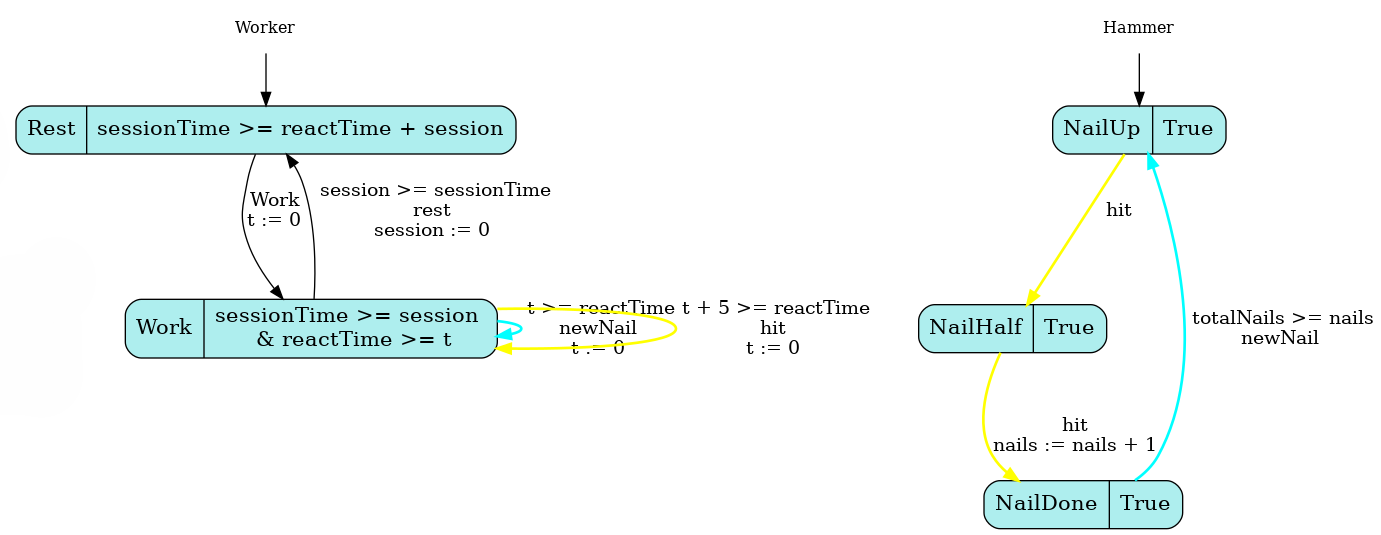
\includegraphics[width=1\linewidth]{images/WH-PTA.png}
    \caption[Worker and Hammer Automata]{Worker and Hammer Automata}
    \label{fig:cof_output}
\end{figure}




\subsubsection{System Analysis}

As before, we start by determining the parameter values needed to avoid a deadlock. In other words, we analyze how the worker's working time, the time required to hammer or place a new nail, and the number of nails must be set to prevent this situation. The property, as previously mentioned, is stored in a separate \texttt{.imiprop} file and has the following syntax: \texttt{property := synth DeadlockFree;} Analyzing the \texttt{.res} file, the parametric interval that guarantees the absence of deadlock is as follows:

\begin{verbatim}
     0 > reactTime
    & sessionTime >= 0
    OR
      reactTime >= sessionTime
    & sessionTime >= 0
\end{verbatim}

We can also determine the parametric interval that guarantees the completion of the worker's action—that is, ensuring that the location NailDone in the Hammer automaton is reachable. For this, we use a simple Reachability property with the following syntax: \texttt{property := \#synth EF(loc[Hammer] = NailDone);}

The parametric interval is of the form:

\begin{verbatim}
     reactTime >= 0
    & sessionTime >= reactTime
\end{verbatim}

To ensure that the completion of the action is guaranteed, reactTime must be a positive value, and additionally, it must be ensured that sessionTime is always greater than or equal to reactTime. Table \ref{tab:property_results} summarizes the verified properties and their corresponding synthesis results. The first property ensures that the system avoids deadlock by constraining the parameters \texttt{reactTime} and \texttt{sessionTime}. The second property determines the conditions under which the system can reach the target location \texttt{cdone}, ensuring progress towards the completion of the task. Together, these results confirm that the model behaves correctly within the specified parameter ranges.


\begin{table}[h!]
\centering
\resizebox{\textwidth}{!}{
\begin{tabular}{|p{5cm}|l|p{5cm}|}
\hline
\textbf{Property} & \textbf{Meaning} & \textbf{Result} \\ \hline
\texttt{property := synth DeadlockFree;} & Ensures the system does not reach a deadlock state. & 
\begin{minipage}[t]{8cm}
$reactTime > 0  \\
\land sessionTime \geq 0$\\
\textbf{or}\\
$sessionTime \geq reactTime \\
\land sessionTime \geq 0$
\end{minipage} \\ \hline

\texttt{property := \#synth EF(loc[Hammer] = NailDone);} & Finds the minimum value of $p_1$ to reach location \texttt{cdone}. &
\begin{minipage}[t]{8cm}
$reactTime \geq 0$\\
$\land sessionTime \geq reactTime$\\
\end{minipage} \\ \hline
\end{tabular}
}
\caption{Synthesis of properties and corresponding results.}
\label{tab:property_results}
\end{table}


\subsection{ATM Machine}

The final example is of a simple ATM with only two functions: balance inquiry and cash withdrawal, considering time constraints for each phase of the operation. The example was also taken from the official Imitator website \cite{IMITATOR}. We begin by declaring the system's variables and clocks:

%\begin{figure} [H]
%    \centering
%    
\includegraphics[width=0.4\linewidth]{images/ATM.jpg}
%    \caption[ATM Machines.]{ATM Machine.\cite{amisb2018atm}}
%    \label{fig:ATM_IMI}
%\end{figure}

%\paragraph{}
\begin{lstlisting}[language=UPPAAL]
    var
    x,y,z : clock;

    p1 : parameter;
    p2 : parameter;
    p3 : parameter;
\end{lstlisting}


Clock x controls the duration of each operation and is used to limit the time allowed for the selected operation. For example, if x = 15 and the chosen operation is withdraw, the user has 15 time units to complete it. Clock y is responsible for tracking the login time, i.e., the time the user takes to provide access credentials.
Finally, clock z monitors the total session time (login + operations). Regarding the variables, they are all defined as parameters: p1 is the maximum allowed session time, p2 defines the maximum time for login, and p3 sets the maximum time allowed per operation, whether it is a balance inquiry or a withdrawal.

\begin{lstlisting}[language=UPPAAL]
    automaton pta
    
    synclabs: ;

    loc Idle: invariant True
    	when True do {x := 0 , y := 0 , z := 0} goto Start;
    
    loc Start: invariant z <= p1
    	when z = p1 goto Idle;
    	when z <= p1 do { y := 0 } goto Login;
    
    loc Login: invariant y <= p2 && z <= p1
    	when z = p1 goto Idle;
    	when True do {x := 0} goto Withdrawals;
    	when y = p2 goto Start;
    	when True do {x := 0} goto Check;
    
    loc Withdrawals: invariant x <= p3
    	when True goto Login;
    
    loc Check: invariant x <= p3
    	when True goto Login;
    
    end
\end{lstlisting}


The automaton is composed of five locations: Idle, Start, Login, Withdrawals, and Check. The initial state is Idle, which represents the ATM being in a standby state, waiting for the start of an operation. When this occurs, all clocks are reset to 0 and the automaton transitions to the Start location. This location marks the beginning of the user interaction. The invariant z <= p1 limits the session duration, with p1 representing the maximum session time; if this limit is exceeded, the system returns to the Idle state (standby). Otherwise, it proceeds to the Login state, where clock y is reset. This clock tracks the time the user takes to log in. In this location, the machine waits for the user to enter their credentials, with the constraint that the login duration must not exceed either of the specified time bounds, as indicated by the invariant \texttt{y <= p2 \&\& z <= p1}. If both conditions are satisfied, the system moves to the Withdrawals location if that was the selected function, or to Check otherwise. In both cases, clock x is reset. If the selected operation is Withdrawal, the system transitions to that location, giving the user a limited time to complete the withdrawal, which cannot exceed p3, as shown by the invariant \texttt{x <= p3}. If the option is Check, it moves to the corresponding location, where the same time restriction applies, also enforced by the invariant \texttt{x <= p3}. In both cases, after completing the action, the system returns to the Login location, allowing the user to repeat or change the selected operation. As with the previous examples, we can construct a transition table for the system, as shown in Figure \ref{tab:atm_tt}.

\begin{table}[h!]
\centering
\resizebox{\textwidth}{!}{
\begin{tabular}{|l|l|l|l|l|l|}
\hline
\textbf{State}         & \textbf{Invariant}                        & \textbf{Guard}          & \textbf{Synchronized Event} & \textbf{Action}                & \textbf{Next State}   \\ \hline
\texttt{Idle}          & Always (\texttt{True})                   & Always (\texttt{True})  & \texttt{start}              & \texttt{x := 0, y := 0, z := 0} & \texttt{Start}        \\ \hline
\texttt{Start}         & $z \leq p_1$                              & $z = p_1$               & \texttt{timeout}            & None                           & \texttt{Idle}         \\ \hline
\texttt{Start}         & $z \leq p_1$                              & $z \leq p_1$            & \texttt{proceed}            & \texttt{y := 0}                & \texttt{Login}        \\ \hline
\texttt{Login}         & $y \leq p_2 \wedge z \leq p_1$            & $z = p_1$               & \texttt{timeout}            & None                           & \texttt{Idle}         \\ \hline
\texttt{Login}         & $y \leq p_2 \wedge z \leq p_1$            & $y = p_2$               & \texttt{restart}            & None                           & \texttt{Start}        \\ \hline
\texttt{Login}         & $y \leq p_2 \wedge z \leq p_1$            & Always (\texttt{True})  & \texttt{withdraw}           & \texttt{x := 0}                & \texttt{Withdrawals}  \\ \hline
\texttt{Login}         & $y \leq p_2 \wedge z \leq p_1$            & Always (\texttt{True})  & \texttt{check}              & \texttt{x := 0}                & \texttt{Check}        \\ \hline
\texttt{Withdrawals}   & $x \leq p_3$                              & Always (\texttt{True})  & \texttt{done}               & None                           & \texttt{Login}        \\ \hline
\texttt{Check}         & $x \leq p_3$                              & Always (\texttt{True})  & \texttt{done}               & None                           & \texttt{Login}        \\ \hline
\end{tabular}
}
\caption{Transition table of the ATM automaton.}
\label{tab:atm_tt}
\end{table}

Finally, we define the parameter constraints and the initial location of the automaton.

\begin{lstlisting}[language=UPPAAL]
    init := 

    & loc[pta] = Idle,
    
    & x = 0
    & y = 0
    & z = 0

    & p1 >= 0
    & p2 >= 0
    & p3 >= 0
    ;

    end
\end{lstlisting}


As mentioned, the system starts in the Idle location, which represents the standby state. Additionally, the only constraint imposed on the parameters is that they must be greater than 0. As with the previous examples, we can convert the model into a figure, as shown in Figure \ref{fig:ATM_output}.


\begin{figure} [H]
    \centering
    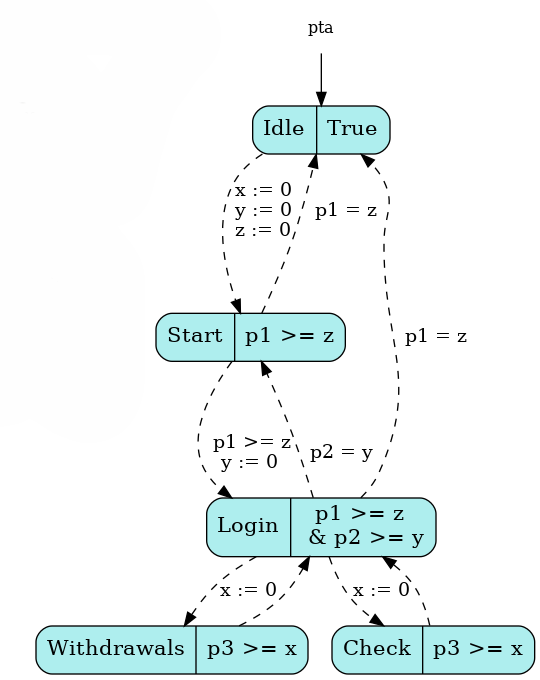
\includegraphics[width=0.6\linewidth]{images/fixed.png}
    \caption[ATM Automata]{ATM Automata}
    \label{fig:ATM_output}
\end{figure}

\subsubsection{System Analysis}

As in the previous examples, the first property to be verified is deadlock-freedom, ensuring that the system does not reach any state from which execution cannot proceed. The syntax for this property, as previously mentioned, is: \texttt{property := synth DeadlockFree}. The parametric interval that guarantees the verification of the property is as follows:

\begin{verbatim}
    p3 >= 0
    & p2 >= 0
    & p1 >= 0
\end{verbatim}

It tell that whatever values the parameters may take, it must be ensured that they are always positive in order to guarantee that "regardless of the situation, the system always has an action to take."

The next property to be verified is a liveness property that searches for at least one cycle in the automaton that goes through the Withdrawals state and can be executed infinitely (i.e., without deadlock). In practical terms, this ensures that it is always possible to perform withdrawals. For this purpose, we use the CycleThrough algorithm, which was briefly mentioned in the previous chapter. The corresponding syntax is: \texttt{property := synth CycleThrough(loc[pta] = Withdrawals);}. The returned parametric interval guarantees that the cycle exists for any non-negative values of parameters p1, p2, and p3.

\begin{verbatim}
    p3 >= 0
    & p2 >= 0
    & p1 >= 0
\end{verbatim}

Additionally, Imitator provides extra information such as the depth at which the cycle was found (i.e., the number of transitions required to complete it), as well as the number of states generated and effectively explored during the analysis.

A summary of the analyzed properties and their corresponding results can be found in Table \ref{tab:property_results_atm}.

\begin{table}[h!]
\centering
\resizebox{\textwidth}{!}{
\begin{tabular}{|p{5cm}|l|p{2cm}|}
\hline
\textbf{Property} & \textbf{Meaning} & \textbf{Result} \\ \hline
\texttt{property := \#synth DeadlockFree;} &
    Ensures the system does not reach a deadlock state. & 
    \begin{minipage}[t]{8cm}
    $p_1 > 0  \\
    \land p_2 \geq 0\\
    \land p_3 \geq 0$\\
    \end{minipage}
\\\hline

\texttt{property := \#synth CycleThrough(loc[pta] = Withdrawals);} & Find a cycle in which the Withdrawals location is visited. \texttt{cdone}. &
\begin{minipage}[t]{4cm}
$p_1 > 0  \\
\land p_2 \geq 0\\
\land p_3 \geq 0$\\
\end{minipage} \\ \hline
\end{tabular}
}
\caption{Synthesis of properties and corresponding results.}
\label{tab:property_results_atm}
\end{table}
























\paragraph{}
\paragraph{}


%\begin{itemize}
%  \item Months 1-3 (Modeling): Using IMITATOR to model and verify 1 or more real-time systems, and to optimize some parameter.


%  expluc do ponto modelig
  
%  \item Months 4-7 (IMITATOR Back-end): Scala development of an Uppex extension to verify real-time families with IMITATOR.
  
%  \item Months 5-9 (Excel DSL): Propose a way to describe parameter optimizations in Excel, aligned with IMITATOR.
  
%  \item Months 7-10 (DSL Back-end): Continue to develop in Scala this extension of Uppex to support the DSL in Excel related to parameter optimization, or other features supported by IMITATOR.
  


%\end{itemize}


